\chapter{Datasets and MonteCarlo samples}
\label{ch:5_2}

% **************************** Define Graphics Path **************************
\ifpdf
    \graphicspath{{Chapter5_2/Figs/Raster/}{Chapter5_2/Figs/PDF/}{Chapter5_2/Figs/}}
\else
    \graphicspath{{Chapter5_2/Figs/Vector/}{Chapter5_2/Figs/}}
\fi

\section{Datasets}

The datasets used in this analysis are listed in Table~\ref{tab:datasets}. These
include the primary signal sample datasets, named `HTMHTParked', for which only
Run2012A is absent as the parked trigger was present only during the 
run period's B, C and D. All other datasets contain events from triggers used for 
background estimation.

\begin{table}[ht]
  \caption{8 \tev Datasets.}
  \label{tab:datasets}
  \centering
  \scriptsize
  \begin{tabular}{ lc }
    \hline
    \hline
    Dataset & Luminosity (fb$^{-1}$) \\
    \hline
    \verb!/HTMHTParked/Run2012B-22Jan2013-v1/AOD! & 4.41 \\
    \verb!/HTMHTParked/Run2012C-22Jan2013-v1/AOD! & 6.80 \\
    \verb!/HTMHTParked/Run2012D-22Jan2013-v1/AOD! & 7.29 \\
    \multicolumn{1}{r}{Total} & 18.49 \\ [0.5ex]
    % \verb!/HT/Run2012A-22Jan2013-v1/AOD! & n/a \\
    \verb!/JetHT/Run2012B-22Jan2013-v1/AOD! & 4.39 \\
    \verb!/JetHT/Run2012C-22Jan2013-v1/AOD! & 6.80 \\
    \verb!/JetHT/Run2012D-22Jan2013-v1/AOD! & 7.29 \\
    \multicolumn{1}{r}{Total} & 18.48 \\ [0.5ex]
    \verb!/SingleMu/Run2012A-22Jan2013-v1/AOD! & 0.69 \\
    \verb!/SingleMu/Run2012B-22Jan2013-v1/AOD! & 4.40 \\
    \verb!/SingleMu/Run2012C-22Jan2013-v1/AOD! & 6.77 \\
    \verb!/SingleMu/Run2012D-22Jan2013-v1/AOD! & 7.27 \\
    \multicolumn{1}{r}{Total} & 19.13 \\ [0.5ex] % 19.13
    \verb!/Photon/Run2012A-22Jan2013-v1/AOD! & 0.68 \\
    \verb!/SinglePhoton/Run2012B-22Jan2013-v1/AOD! & 4.40 \\
    \verb!/SinglePhoton/Run2012C-22Jan2013-v1/AOD! & 6.77 \\
    \verb!/SinglePhotonParked/Run2012D-22Jan2013-v1/AOD! & 7.27 \\
    \multicolumn{1}{r}{Total} & 19.12 \\ [0.5ex] % 19.18
    \hline
    \hline
  \end{tabular}
\end{table}

\section{MonteCarlo Background and Signal samples}

The full list of MonteCarlo (MC) samples used in this analysis are listed in 
Table~\ref{tab:mc-sm} along with the number of events, next-to-next-to-leading 
order (NNLO) cross section and an effective integrated luminosity for each.

\emph{can describe the different methods of MC generation}
The Parton Density Functions (PDF) of colliding protons are modelled according
to the
CTEQ6L1 distribution, the matrix-element level hard-scatter performed by
\MADGRAPH or \PYTHIA, with any outgoing partons showered in \PYTHIA. The
produced generator level particles are then put through a full detector
simulation in \GEANT, and detector hits `digitized' in order to simulate the
response of detector electronics. Prior to digitization, a number of
`MinimumBias' events are
over-layed in order to reproduce LHC run conditions. Event-level weights
are applied to each simulated sample such that both the PU and equivalent
integrated luminosity are matched to a given data sample.

Additional corrections are made to simulated event samples in order to correct
the efficiency of b-tagging algorithms to match that seen in data. Corrections
are determined as a function of jet-flavour (light/c/b), defined as:

\begin{equation}
SF_{light,c,b} = \frac{\epsilon^{data}_{light,c,b}(\Pt, \eta)}{\epsilon^
{MC}_ {light,c,b}(\Pt, \eta)}
\end{equation}

where $\epsilon^{X}_{light, c, b}$ represents \Pt and $\eta$ dependent
b-tagging efficiencies measured in data and MC.

\begin{landscape}
  \begin{center}
    \begin{table}[ht]
      \caption{MC samples for Standard Model processes.}
      \label{tab:mc-sm}
      \centering
      \tiny
      \begin{tabular}{ lrrrr }
        \hline
        Sample & N$_{\textrm{event}}$ & Cross section (pb) & Corrected Cross section (pb) & Luminosity (fb$^{-1}$) \\
        \hline
        \hline
        \verb!/WJetsToLNu_TuneZ2Star_8TeV-madgraph-tarball/Summer12_DR53X-PU_S10_START53_V7A-v1/AODSIM!           & 57661905 & 37509.0 & 34133.2 & 1.5     \\
        \verb!/WJetsToLNu_HT-150To200_8TeV-madgraph/Summer12_DR53X-PU_S10_START53_V7C-v1/AODSIM!                  & 21414209 & 253.8   & 234.53  & 84.4    \\
        \verb!/WJetsToLNu_HT-200To250_8TeV-madgraph/Summer12_DR53X-PU_S10_START53_V7C-v1/AODSIM!                  & 9895771  & 116.5   & 103.94  & 84.9    \\
        \verb!/WJetsToLNu_HT-250To300_8TeV-madgraph_v2/Summer12_DR53X-PU_S10_START53_V7A-v1/AODSIM!               & 4924990  & 57.6    & 51.34   & 85.5    \\
        \verb!/WJetsToLNu_HT-300To400_8TeV-madgraph_v2/Summer12_DR53X-PU_S10_START53_V7A-v1/AODSIM!               & 5141023  & 48.4    & 42.41   & 106.2   \\
        \verb!/WJetsToLNu_HT-400ToInf_8TeV-madgraph_v2/Summer12_DR53X-PU_S10_START53_V7A-v1/AODSIM!               & 4923847  & 30.8    & 26.36   & 159.9   \\
        \verb!/ZJetsToNuNu_50_HT_100_TuneZ2Star_8TeV_madgraph(_ext)/Summer12_DR53X-PU_S10_START53_V7A-v1/AODSIM!  & 23743998 & 452.8   & 405.21  & 52.4    \\
        \verb!/ZJetsToNuNu_100_HT_200_TuneZ2Star_8TeV_madgraph(_ext)/Summer12_DR53X-PU_S10_START53_V7A-v1/AODSIM! & 9876059  & 190.4   & 173.76  & 51.9    \\
        \verb!/ZJetsToNuNu_200_HT_400_TuneZ2Star_8TeV_madgraph(_ext)/Summer12_DR53X-PU_S10_START53_V7A-v1/AODSIM! & 9649619  & 45.1    & 42.41   & 214.0   \\
        \verb!/ZJetsToNuNu_400_HT_inf_TuneZ2Star_8TeV_madgraph(_ext)/Summer12_DR53X-PU_S10_START53_V7A-v1/AODSIM! & 5079710  & 6.26    & 5.81    & 811.5   \\
        \verb!/TT_CT10_TuneZ2star_8TeV-powheg-tauola/Summer12_DR53X-PU_S10_START53_V7A-v1(v2)/AODSIM!             & 27094723 & 234.0   & 271.44  & 115.8   \\
        \verb!/TTZJets_8TeV-madgraph_v2/Summer12_DR53X-PU_S10_START53_V7A-v1/AODSIM!                              & 210160   & 0.172   & 0.172   & 1221.9  \\
        \verb!/T_t-channel_TuneZ2star_8TeV-powheg-tauola/Summer12_DR53X-PU_S10_START53_V7A-v1/AODSIM!             & 3710227  & 56.4    & 56.4    & 65.8    \\
        \verb!/Tbar_t-channel_TuneZ2star_8TeV-powheg-tauola/Summer12_DR53X-PU_S10_START53_V7A-v1/AODSIM!          & 1935072  & 30.7    & 30.7    & 63.0    \\
        \verb!/T_s-channel_TuneZ2star_8TeV-powheg-tauola/Summer12_DR53X-PU_S10_START53_V7A-v1/AODSIM!             & 243961   & 3.79    & 3.79    & 64.4    \\
        \verb!/Tbar_s-channel_TuneZ2star_8TeV-powheg-tauola/Summer12_DR53X-PU_S10_START53_V7A-v1/AODSIM!          & 139974   & 1.76    & 1.76    & 79.5    \\
        \verb!/T_tW-channel-DR_TuneZ2star_8TeV-powheg-tauola/Summer12_DR53X-PU_S10_START53_V7A-v1/AODSIM!         & 497658   & 11.1    & 11.1    & 44.8    \\
        \verb!/Tbar_tW-channel-DR_TuneZ2star_8TeV-powheg-tauola/Summer12_DR53X-PU_S10_START53_V7A-v1/AODSIM!      & 493460   & 11.1    & 11.1    & 44.5    \\
        \verb!/DYJetsToLL_M-10To50filter_8TeV-madgraph/Summer12_DR53X-PU_S10_START53_V7A-v1/AODSIM!               & 7116223  & 13124.1 & 12205.4 & 0.5     \\
        \verb!/DYJetsToLL_M-50_TuneZ2Star_8TeV-madgraph-tarball/Summer12_DR53X-PU_S10_START53_V7A-v1/AODSIM!      & 30171503 & 3503.7  & 3258.45 & 8.6     \\
        \verb!/DYJetsToLL_HT-200To400_TuneZ2Star_8TeV-madgraph(_ext)/Summer12_DR53X-PU_S10_START53_V7A-v1/AODSIM! & 6892777  & 24.3    & 22.24   & 283.7   \\
        \verb!/DYJetsToLL_HT-400ToInf_TuneZ2Star_8TeV-madgraph/Summer12_DR53X-PU_S10_START53_V7A-v1/AODSIM!       & 2695789  & 3.36    & 3.11    & 802.3   \\
        \verb!/GJets_HT-200To400_8TeV-madgraph/Summer12_DR53X-PU_S10_START53_V7A-v1/AODSIM!                       & 57891147 & 1140.8  & 1060.9  & 50.7    \\
        \verb!/GJets_HT-400ToInf_8TeV-madgraph/Summer12_DR53X-PU_S10_START53_V7A-v1/AODSIM!                       & 9459562  & 124.7   & 115.97  & 75.9    \\
        \verb!/WW_TuneZ2star_8TeV_pythia6_tauola/Summer12_DR53X-PU_S10_START53_V7A-v1/AODSIM!                     & 9888431  & 57.1    & 57.1    & 173.2   \\
        \verb!/WZ_TuneZ2star_8TeV_pythia6_tauola/Summer12_DR53X-PU_S10_START53_V7A-v1/AODSIM!                     & 9841248  & 12.6    & 12.6    & 781.1   \\
        \verb!/ZZ_TuneZ2star_8TeV_pythia6_tauola/Summer12_DR53X-PU_S10_START53_V7A-v1/AODSIM!                     & 9751908  & 8.26    & 8.26    & 1180.6  \\
        \verb!/QCD_Pt-50to80_TuneZ2star_8TeV_pythia6/Summer12_DR53X-PU_S10_START53_V7A-v2!                        & 5950860  & 8148778 & 8148778 (LO) & 0.001   \\
        \verb!/QCD_Pt-80to120_TuneZ2star_8TeV_pythia6/Summer12_DR53X-PU_S10_START53_V7A-v3!                       & 5962864  & 1033680 & 1033680 (LO) & 0.006   \\
        \verb!/QCD_Pt-120to170_TuneZ2star_8TeV_pythia6/Summer12_DR53X-PU_S10_START53_V7A-v3!                      & 5985732  & 156293  & 156293  (LO) & 0.038   \\
        \verb!/QCD_Pt-170to300_TuneZ2star_8TeV_pythia6/Summer12_DR53X-PU_S10_START53_V7A-v1(v2)!                  & 20155180 & 34138   & 34138   (LO) & 0.590   \\
        \verb!/QCD_Pt-300to470_TuneZ2star_8TeV_pythia6/Summer12_DR53X-PU_S10_START53_V7A-v1(v2,v3)!               & 23588100 & 1759.5  & 1759.5  (LO) & 13.4    \\
        \verb!/QCD_Pt-470to600_TuneZ2star_8TeV_pythia6/Summer12_DR53X-PU_S10_START53_V7A-v2!                      & 3978848  & 113.9   & 113.9   (LO) & 34.9    \\
        \verb!/QCD_Pt-600to800_TuneZ2star_8TeV_pythia6/Summer12_DR53X-PU_S10_START53_V7A-v2!                      & 3964864  & 27.0    & 27.0    (LO) & 146.8   \\
        \verb!/QCD_Pt-800to1000_TuneZ2star_8TeV_pythia6/Summer12_DR53X-PU_S10_START53_V7A-v2!                     & 3854563  & 3.55    & 3.55    (LO) & 1085.8  \\
        \verb!/QCD_Pt-1000to1400_TuneZ2star_8TeV_pythia6/Summer12_DR53X-PU_S10_START53_V7A-v1!                    & 1964088  & 0.738   & 0.738   (LO) & 2661.4  \\
        \verb!/QCD_Pt-1400to1800_TuneZ2star_8TeV_pythia6/Summer12_DR53X-PU_S10_START53_V7A-v1!                    & 1988062  & 0.0335  & 0.0335  (LO) & 59345.1 \\
        \verb!/QCD_Pt-1800_TuneZ2star_8TeV_pythia6/Summer12_DR53X-PU_S10_START53_V7A-v1!                          & 977586   & 0.00183 & 0.00183 (LO) & 534200  \\
        \verb!/QCD_HT-100To250_TuneZ2star_8TeV-madgraph-pythia/Summer12_DR53X-PU_S10_START53_V7A-v1/AODSIM!       & 50081518 & 1.036E7 & 1.036E7 (LO) & 0.005   \\
        \verb!/QCD_HT-250To500_TuneZ2star_8TeV-madgraph-pythia6/Summer12_DR53X-PU_S10_START53_V7A-v1/AODSIM!      & 27062078 & 276000. & 276000. (LO) & 0.1     \\
        \verb!/QCD_HT-500To1000_TuneZ2star_8TeV-madgraph-pythia6/Summer12_DR53X-PU_S10_START53_V7A-v1/AODSIM!     & 27613225 & 8426.   & 8426.   (LO) & 3.3     \\
        \verb!/QCD_HT-1000ToInf_TuneZ2star_8TeV-madgraph-pythia6/Summer12_DR53X-PU_S10_START53_V7A-v1/AODSIM!     & 12018415 & 204.    & 204.    (LO) & 58.9    \\
        \hline
      \end{tabular}
    \end{table}
  \end{center}
\end{landscape}

Interpretations are made using signal MC samples, each representing a scan in 
the phase space of a specific SMS model. The samples used are listed in
Table~\ref{tab:mc-signal}. Each sample is generated at the parton level using \MADGRAPH and then
decayed using \PYTHIASIX \emph{(too vague?)}. Up to two additional partons are simulated 
in the initial generation step to ensure good modelling of initial state 
radiation (ISR), however supplementary samples were produced with up to three
additional partons to allow for systematic studies into the effect on the 
analysis, as detailed in chapter~\ref{ch:9}.

\begin{landscape}
  \begin{center}
    \begin{table}[ht]
      \caption{MC samples for simplified models.}
      \label{tab:mc-signal}
      \centering
      \tiny
      \begin{tabular}{ lll }
        \hline
        Model & Sample & Description \\
        \hline
        \hline
        \verb!T2cc!     & \verb!/SMS-MadGraph_2J_T2cc_NoFilter_mStop-100to250_mLSP-20to230_8TeV-Pythia6Zstar/Summer12-START52_V9_FSIM-v1/AODSIM! & Original scan \\
        \verb!T2cc!     & \verb!/SMS-T2cc_NoFilter_mStop-175to250_mLSP-95to240_8TeV-Pythia6Z/Summer12-START52_V9_FSIM-v1/AODSIM! & Original scan \\
        \verb!T2cc!     & \verb!/SMS-T2cc_2J_mStop-250to350_mLSP-195to340_TuneZ2star_8TeV-madgraph-tauola/Summer12-START53_V19_FSIM-v2/AODSIM! & Scan extension \\
        \verb!T2cc!     & \verb!/SMS-8TeV_Pythia6Z_T2cc_3jets_mStop-200_mLSP-120/Summer12-START52_V9_FSIM-v1/AODSIM! & 3-parton sample \\
        \verb!T2cc!     & \verb!/SMS-8TeV_Pythia6Z_T2cc_3jets_mStop-200_mLSP-190/Summer12-START52_V9_FSIM-v1/AODSIM! & 3-parton sample \\
        \verb!T2degen!  & \verb!/SMS-T2DegenerateStop_2J_mStop-100to150_mLSP-20to140_TuneZ2star_8TeV-madgraph-tauolapp/Summer12-START53_V19_FSIM_PU_S12-v1/AODSIM! & Original scan \\
        \verb!T2degen!  & \verb!/SMS-T2DegenerateStop_2J_mStop-175to225_mLSP-95to215_TuneZ2star_8TeV-madgraph-tauolapp/Summer12-START53_V19_FSIM_PU_S12-v1/AODSIM! & Original scan \\
        \verb!T2degen!  & \verb!/SMS-T2DegenerateStop_2J_mStop-250to300_mLSP-170to290_TuneZ2star_8TeV-madgraph-tauolapp/Summer12-START53_V19_FSIM_PU_S12-v1/AODSIM! & Original scan \\
        \verb!T2degen!  & \verb!/SMS-T2DegenerateStop_2J_mStop-325to375_mLSP-245to365_TuneZ2star_8TeV-madgraph-tauolapp/Summer12-START53_V19_FSIM_PU_S12-v1/AODSIM! & Original scan \\
        \verb!T2degen!  & \verb!/SMS-T2DegenerateStop_2J_mStop-400_mLSP-320to390_TuneZ2star_8TeV-madgraph-tauolapp/Summer12-START53_V19_FSIM_PU_S12-v1/AODSIM! & Original scan \\
        \hline
        \hline
      \end{tabular}
    \end{table}
  \end{center}
\end{landscape}

\section{Correcting SM sample cross sections}
\label{sec:mc_xsec_corrs}

\subsection{\HTpart binned samples}
In order to increase statistics this analysis makes use of MC samples binned in 
parton-level \HT (\HTpart). Leading order (LO) cross-sections are provided with 
these samples, which are translated into next-to-next-to-leading order (NNLO) 
cross-sections using translation-factors (k-factors) derived from corresponding 
inclusive sample cross-sections. However, recent CMS studies (REF) have shown that the 
provided LO cross-sections for \HTpart binned samples can 
be incorrect by up to 10\%. This is shown in figure~\ref{fig:xsec_study_before},
where un-physical steps are present in the ratio between the \zj binned sample 
and the \dyj inclusive sample.

\begin{figure}[b!]
  \centering
  \begin{subfigure}[b]{0.45\textwidth}
    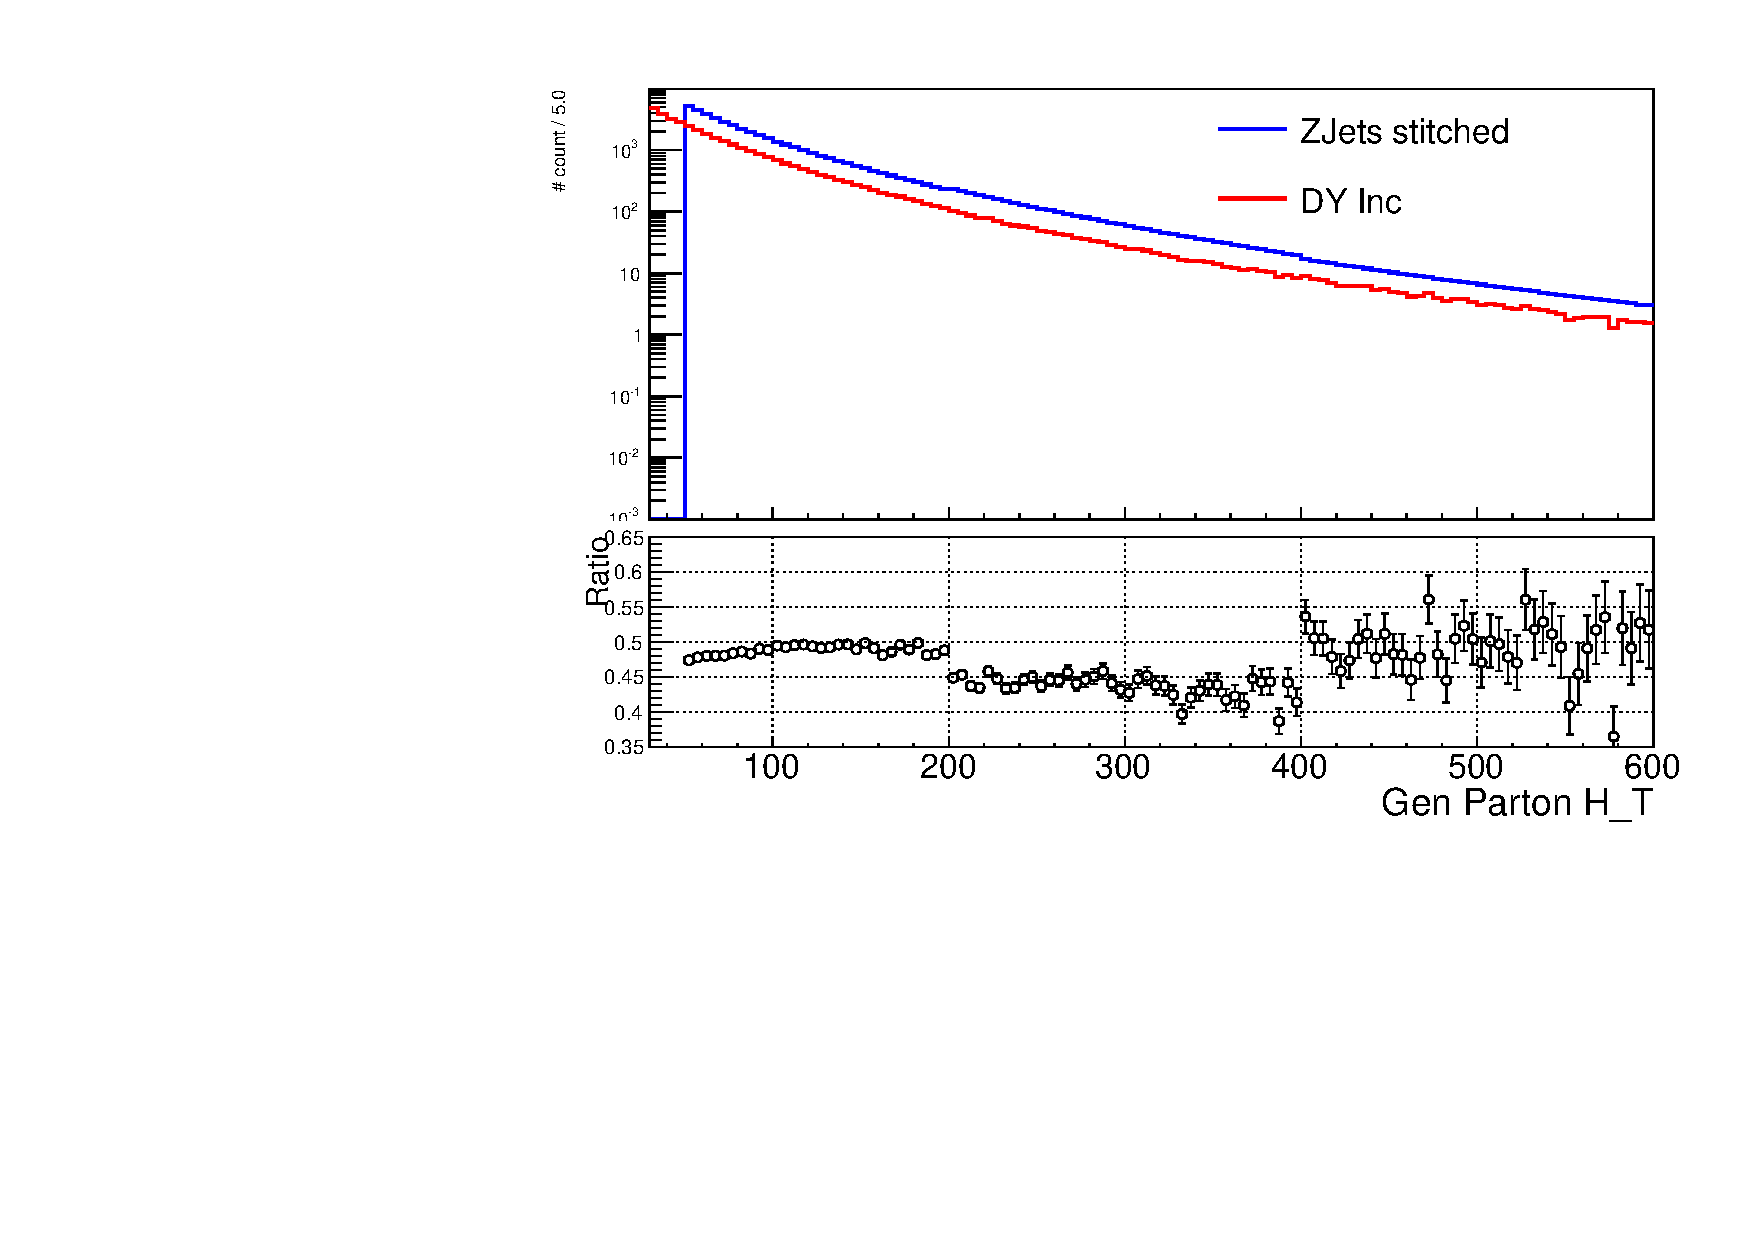
\includegraphics[width=\textwidth]{/Users/chrislucas/SUSY/thesis/Figs/xs_study/compar_genPartonHT_zmass_0_inc_inc_DYZJets_noCuts_sitv_log_HCPxS.pdf}
    \caption{No corrections.}
    \label{fig:xsec_study_before}
  \end{subfigure}             
  \begin{subfigure}[b]{0.45\textwidth}
    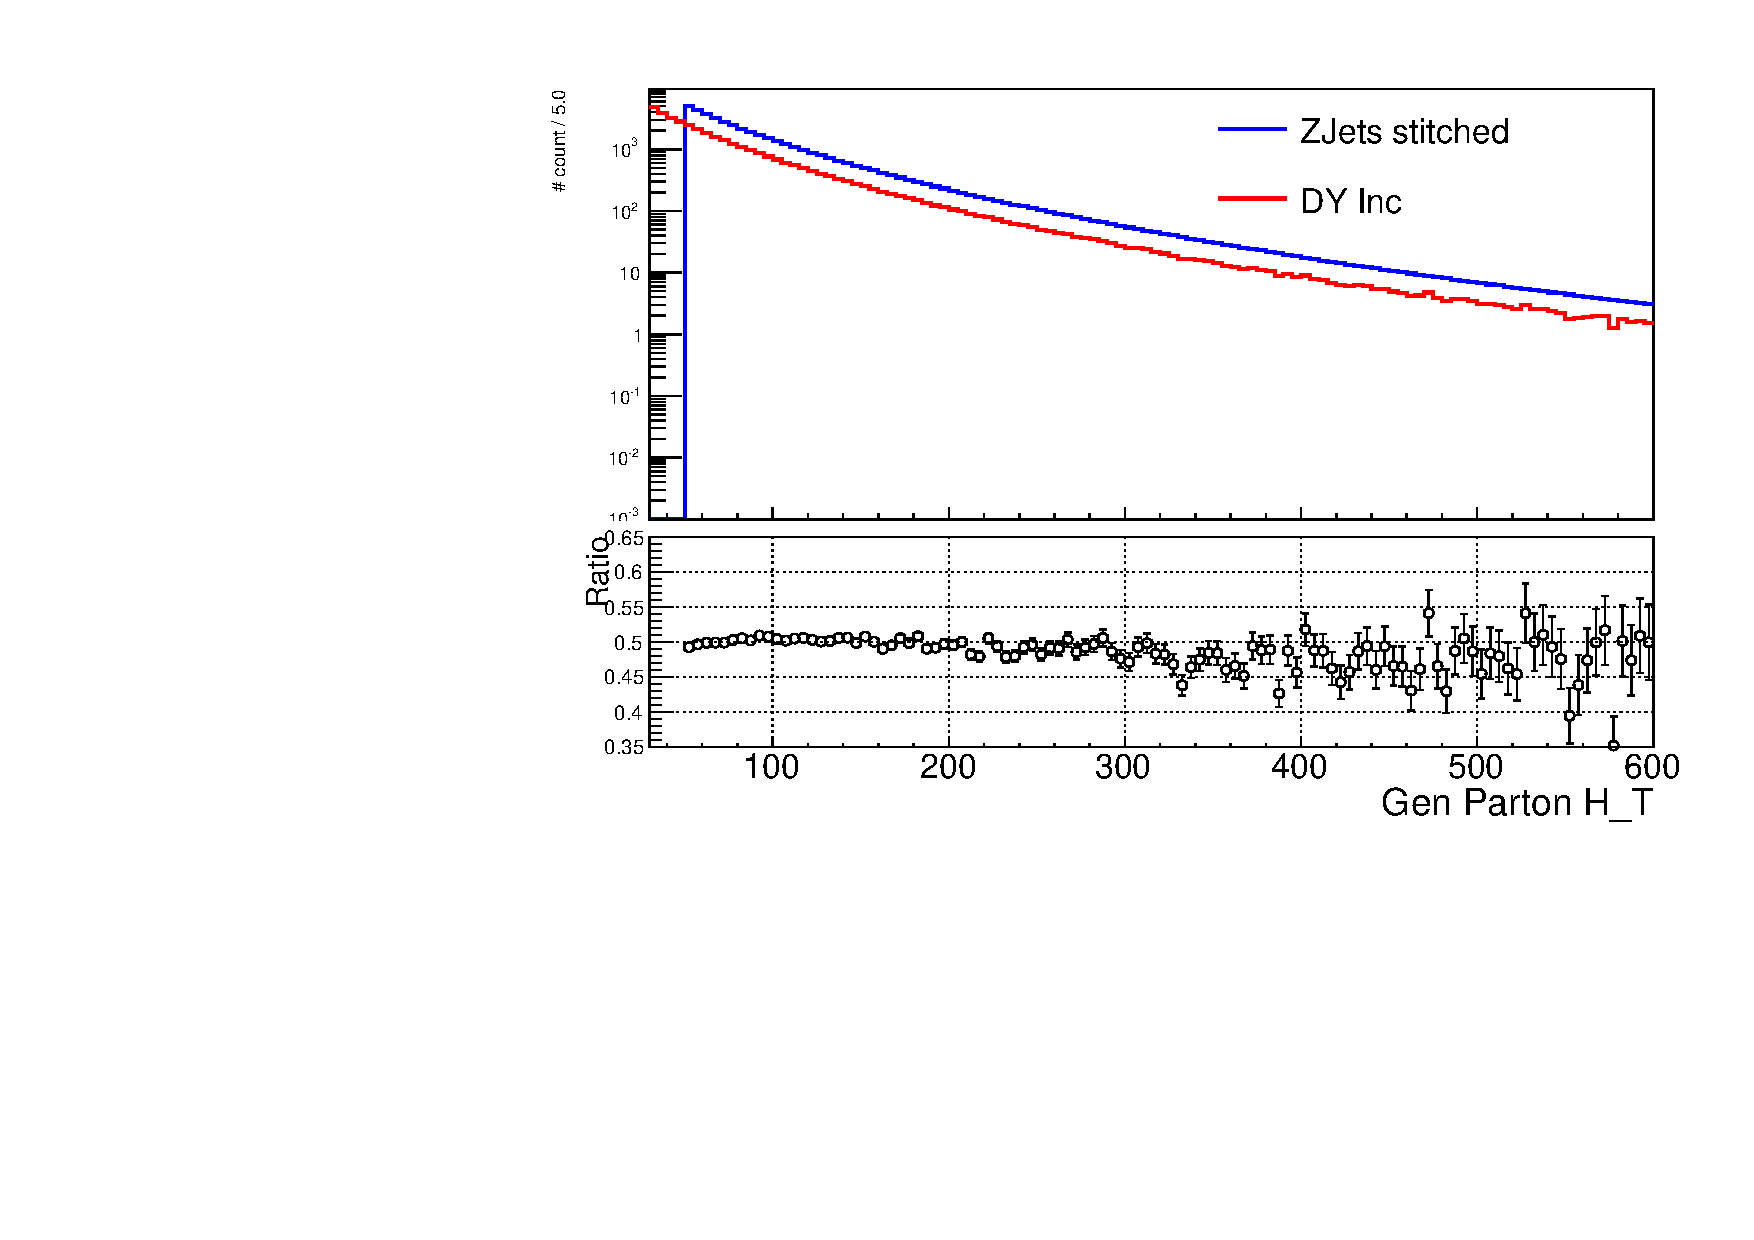
\includegraphics[width=\textwidth]{/Users/chrislucas/SUSY/thesis/Figs/xs_study/compar_genPartonHT_zmass_0_inc_inc_DYZJets_noCuts_sitv_log.pdf}
    \caption{With corrections.}
    \label{fig:xsec_study_after}
  \end{subfigure}             
  \caption{Generator level \HTpart distributions from the
    inclusive DY + jets and the \HTpart binned \zj
    samples.}
  \label{fig:xsec_study}
\end{figure}

Two of the binned samples have corresponding inclusive samples to allow for 
this comparison to be made, namely \wj and \dyj. For these two cases, the 
derivation of corrections for each \HTpart binned sample is simple. However, for 
\zj and \gj, no such inclusive samples exist. These binned samples are 
compared against the inclusive \dyj sample, where the overall normalisation is 
set according to the relative branching fraction of \zinv and GAMMA to
$Z \to \ell\ell$, set as 0.505 and VALUE, respectively. An example ratio plot is
shown in figure~\ref{fig:xsec_study_after}, where a constant ratio between the 
samples is found.


\subsection{HT side-band normalisation}
As mentioned previously in section~\ref{sec:mc_xsec_corrs}, absolute MC 
normalisation is not well modelled in the high-\met region of 
phase-space in which many SUSY analyses search. As such, data and MC appear to
disagree using `out-of-the-box' MC samples and cross-sections. While data and MC
comparisons are not explicitly used in this analysis, ratios of MC yields are, 
and so cross-section correction factors for the main 
MC processes are determined. These are measured as the data to MC ratio in the
$150 \leq \HT < 200$ \gev side-band region, in a given control sample with a 
given selection, designed to produce a pure sample of a background process. A
summary of the selections and their relevant purities are given in table~\ref{tab:ht_sideband}.

\begin{table}[!ht]
  \caption{Correction factors determined from a data side-band for the different
    MC samples. All Correction factors are relative to theoretical cross
    sections calculated at NNLO. The corrections measured for the W +
    jets and Z + jets processes, which are in agreement, are also
    applied to the \zinv + jets and \gj samples. ``Corrected yield''
    reflects the observed data yield minus the contamination as given
    by MC. RE}
  \label{tab:ht_sideband}
  \centering
  \small
  \begin{tabular}{ llcc }
    \hline
    \hline
    Process                       & Selection                         & Purity & Correction factor        \\
    \hline
    W + jets                      & \mj, \njlow, $\nb = 0$          & 0.91   & $0.93 \pm 0.01$ \\
    Z($\rightarrow\mu\mu$) + jets & \mmj, \njlow, $\nb = 0$         & 0.98   & $0.94 \pm 0.04$ \\
%    \ttbar                       & \mj, $\nj \geq 2$, $\nb \geq 2$ & 0.73   & $1.25 \pm 0.05$ \\
    \ttbar                        & \mj, $\nj \geq 2$, $\nb \geq 2$ & 0.87   & $1.21 \pm 0.05$ \\ % includes single top
    \hline
    \hline
  \end{tabular}
\end{table}

These derived correction factors are tested in the closure tests performed
following their application (section~\ref{sec:closure_tests}).
